\documentclass[gaiyou]{hitsotsuron} %文書のクラスファイルを指定

%題目の各文字列を指定
\title{カード操作方式に基づくプログラミング学習支援システムのフィードバック機能の現状分析及び改善に関する研究}

\papertype{令和5年度卒業研究成果報告}
\author{森俊介}
\snumber{BL19103}
\advisor{松本 慎平}
\date{2023年1月13日}

\begin{document} %文書本体の開始

%題目を実際に作成
\twocolumn[%
\maketitle
]

\if0

Latexの利用に関する参考URL)

LaTeX - コマンド一覧
http://www1.kiy.jp/~yoka/LaTeX/latex.html

LaTeXコマンドシート一覧
https://members.tripod.com/e_luw/gakko/latex1/l_list.html

\fi

% 緒言
\section{緒言}

意味のある部分間の関係を考えるプログラミング学習において,課題外在性負荷を減らすため,カード操作方式による学習支援システム(Card Operation-Based Programming Learning Support System,以降,COPS)が開発されている\cite{matsumoto2018}.大学講義で従来システムを導入した結果,非本質的な認知負荷を減らしながら,教授者が意図した学習活動に集中できていたこと,とりわけ初学者にとって有効な学習方法であることが示唆された.また,従来のシステムは,従来のコーディング主体の学習とは同等の学習効果を有しながら,従来よりも学習時間を短縮できる効率的な学習方法であることが明らかにされた.一方,先行研究の中で,COPSの学習の質を評価するため,学習ログデータを知識工学の考え方に基づき分析したところ,適切な学習活動を行っていない学習者の存在が確認された.具体的には,知識を用いず,フィードバックとして与えられたヒントのみを頼りに網羅的に探索すること(知識無し解法)の合理性が示唆された.このような結果が得られた理由は様々考えられるが,可能性の一つとして,既存のフィードバック機能の設計に原因があったのではないかと先行研究によって指摘された.COPSでは,学習者が回答した際,「プログラムの実行結果」や「正誤のフィードバック」と共に,「カード配置の適切さ」の3つの情報が学習者に通知される.これら3つのうち,「カード配置の適切さ」について,必要以上の手助けを行っていたために,試行錯誤的なカード順列の設置・繰り返しが合理的戦略であった可能性が高く,適切な学習の妨げになっていたと結論付けられていた.ただし,この結論はあくまで推測に過ぎない.そこで本研究では,「カード配置の適切さ」に関するフィードバック方式の適切性を実験的に明らかにすることを目的とする.

% 実験方法の提案
\section{先行研究}
COPSは,問題文とプログラムコードの書かれたカードを提示し,カードを並び替えてるプログラムを組み立てる学習を支援するWeb アプリケーションである.カードは,マウス操作で動かすことができる. 

COPSでは,「カード順列の適切さ」を3パターンの色で学習者にフィードバックし足場掛けを試みている.具体的には,正誤確認やコンパイルを行った時,回答欄に設定されたカードの選択と位置が共に正しければ青色,カードの選択のみ正しく場所が間違っていれば黄色,ダミーカードが選択されていれば赤色がカードに表示される.学習者はこの3色を手掛かりに,正解とのギャップを確認できるようになっている.「カード順列の適切さ」を用いたCOPSの既存のフィートバック機能自体の有用性については,森永の研究\cite{morinaga2019new}で明らかにされている.ただし,森永の研究では,あくまで学習者にとって適切な難易度の課題が与えられることが前提とされている.この点に着目し,姫井は,知識無し解法の合理性は課題の難易度が学習者にとって高すぎる場合にのみ見られる傾向だと仮定し,この仮説を明らかにすることを目的として研究を進めた.その結果,高難易度の問題が与えられた際,「カード配置の適切さ」に関するフィードバックを行った群のコンパイル回数や正誤診断の回数がそうでない群に加えて有意に高く,姫井の仮説を裏付ける結果が明らかにされた.ただし,「カード配置の適切さ」のフィードバックについては,学習者に対するインタビュー評価から,足場掛けとして有用であることが示されている.そのため,「カード配置の適切さ」のフィードバック自体を取りやめるのではなく,既存の方法を改善した方法の構築が必要だと言える.

\section{提案}

\if0

従来システムに焦点を当てた先行研究では,学習者自身が正解までの近さを把握可能なフィードバック方式を提案し,知覚的喚起に有効であること,行間の活動に認知資源を集中出来ていることを実験で明らかにした\cite{morinaga2019new}.以上から,フィードバック機能は有用であると結論づけた.

森永らの実験では,実行結果とSIEM理論に基づいたフィードバックを受ける群,実行結果だけを得る統制群の2群に被験者を10名ずつ分けて比較実験を行った.実験の結果,事後試験の平均で実験群は3.52点,統制群は平均3,41点であった.この結果では統計的に有意な差は得られなかったが,アンケート結果は``動作確認を見るのは楽しいか?''といった項目で実験群の方がt検定(両側)で有意($p<.05$)に高かった.この結果から,フィードバックで学習効果の低下など見られなかったため学習方式として問題ないこと,高い主観評価から学習意欲が高まり学習の持続が期待できると結論付けた.以上より,持続的に学習させるためには,実行結果と共に自分の立ち位置を意識させることが有効であることを確認した.一方,学習者の回答から得られた出力パターンを入力とし,そこから正解までの近さを自動的に判定する機能は開発されていない.現在の段階では,正解までの近さを示した出力パターン一覧を学習者は事前に受け取っており,それに基づいて,学習者は自ら正解までの近さを判断しなければならない.よってこの開発は学習効率の向上に有用であると考えられる.

\fi

本研究では,「カード配置の適切さ」について,%段階的開発学習を支援するためのフィードバック機能は従来システムのそれと比べて学習効果の観点から有用かどうかを明らかにする.段階的開発学習とは,課題全体の一部の要件のみを取り出した部分問題を定義し,その部分問題のプログラム開発を繰り返すことによって,全体の課題解決を目指す開発戦略を意味する.この段階的開発学習を支援するためには,
回答欄に設定されたカードが正しいか/そうでないか,のみのフィードバックの有用性を調査する.
%なお,段階的詳細化法\cite{wirth2001program}での学習も支援したいと考えている.それを行うためには, テスト実行時に用いられる「スタブ」と同様の役割を持つカードを用意することで可能だと考えている.
具体的には,正誤確認やコンパイルを行った時,回答欄に設定されたカードの選択が正しければ青色,ダミーカードが選択されていれば赤色,の2色のみのフィードバックを行う.先行研究のフィードバックの青と黄の2色を合わせて,回答に設定されたカードの選択が正しい場合を青とすることによって,色のフィードバック情報のみを頼りに網羅的探索を行うことが難しくなると想定している.その有用性については,比較実験を行い明らかにする予定である.その他の取り組みとして,操作ログデータを分析することによって,試行錯誤的な操作量の定量化に取り組む予定である.そして,定量化されたデータに基づいて,「カード配置の適切さ」のフィードバックの違いが試行錯誤量低減に対する有用性を数量的に明らかにしていく.

%一方,姫井の研究によって,従来システムのフィードバック機能の特性が明らかになった場合であっても,フィードバックの手法自体を見直すものではない.学習者の理解度は相対的に変化するものである.よって,知識無し探索を合理的戦略として適用する学習者を減らすことは,姫井の研究だけでは難しい.そこで本研究では,従来システムのフィードバック機能を見直し,段階的開発活動を支援する程度のフィードバック機能を新たに提案する.そして,提案法の有用性を実験的に明らかにする.

\section{実験方法}

被験者は,情報学を学ぶ大学生3,4年生とし,理解度を図るプレテストを行い,学力水準が平等になるように実験群と統制群に分ける.一方提案システムでは,回答欄に設定されたカードの選択が正しければ青,そうでなければ赤とする.これらフィードバックの学習効果及び主観評価の差を実験で明らかにする.具体的には,本研究のフィードバックが先行研究のフィードバックより,フィードバック利用回数が少なくなることにより,網羅的探索をしている可能性が減っていることを予定している.実験後,ポストテストと共にアンケートを実施し,動機付けの効果や認知負荷を調査する.

%ARCSモデル
%認知負荷を評価するアンケート

\if0

\section{実験方法}

被験者は,情報学を学ぶ大学生3,4年生とし,理解度を図るプレテストを行い,学力水準が平等になるように実験群と統制群に分ける.一方提案システムでは,回答欄に設定されたカードの選択が正しければ青,そうでなければ赤とする.これらフィードバックの学習効果及び主観評価の差を実験で明らかにする.実験後,ポストテストと共にアンケートを実施し,動機付けの効果や認知負荷を調査する.

\fi

%分析結果
\section{分析結果}
実験後,分析を行った結果,下の図に示すように,テスト2,3ではフィードバック利用回数が減少したとともに,テスト1,3の統制群にあった外れ値が実験群では無くなった.
ポストテストの結果では,テスト1では有意な結果が得られなかったが,テスト2,3では統制群に比べ実験群の方が点数が高くなった.さらに,T検定を行ったの結果,テスト3ではp<0.1となったため,有意傾向にあることが分かった.
認知負荷アンケートでは,統制群より実験群の方が色情報によるヒントが減少しているため,実験群の方が内在性負荷・外在性負荷において高くなったため,複雑であるという結果が得られた.学習関連負荷の項目では,テスト1はほとんど変化がなかったが,テスト2,3では実験群の方が高くなったため,学習に役立ったことが分かった.
フロー理論アンケートでは,学習の増加において有意である結果が得られたため,学習者は学習したという実感が得られていることが分かった.
テスト2,3のフィードバック利用回数の減少,ポストテスト3がp<0.1となり有意傾向にある,アンケートの結果から学習した実感が得られているというこの3点から難易度の高い問題において本研究の2色のフィードバックは有用であるといえる.

\begin{figure}[tb]
	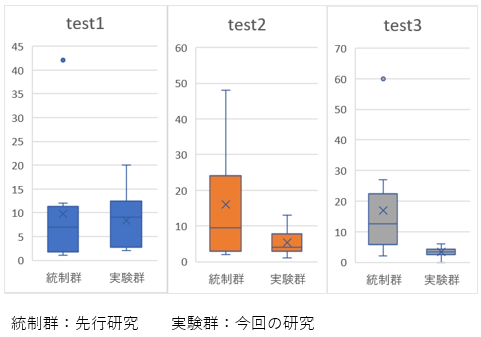
\includegraphics[width=0.9\linewidth]{tex1.png}
	\centering
	\caption{フィードバック利用回数}
	\label{fig1}
\end{figure}

\begin{figure}[tb]
	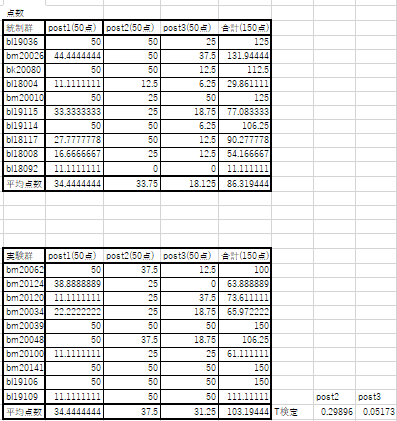
\includegraphics[width=0.9\linewidth]{tex2.png}
	\centering
	\caption{ポストテスト点数・T検定}
	\label{fig1}
\end{figure}

%結言
\section{結言}

本研究では,「カード配置の適切さ」に関するフィードバック方式の適切性を実験的に明らかにする方法を提案し,今後の計画を示した.

\bibliographystyle{junsrt}    % スタイル(bstファイル名)を記述する.jplain,plainはpLaTeXに標準で付いている.
%\nocite{*}                 % 本文中で参照していない文献をリストに載せたい場合に用いる.*を指定すると全て載せる.通常使わないのでコメントアウトしている.
\bibliography{reflist}    % bibファイル名を指定する.拡張子は除く.
\end{document} 
